\begin{appendices}

%
% The first appendix must be "Self-appraisal".
%
\chapter{Self-appraisal}

\section{Critical self-evaluation}

\subsection{Project Scope and Time Management}

Development proceeded more reactively than planned. Rather than defining a comprehensive feature roadmap upfront, work on each component began when it became the immediate bottleneck. This was partly a consequence of the initial Waterfall plan proving too rigid: new algorithmic questions emerged during implementation that required revisiting the background material, making a clean design-then-build separation impractical. The transition toward Agile methodologies was therefore organic, and proved more effective in this context, as short iteration cycles allowed design decisions to incorporate findings from earlier implementation phases.

The most significant scope casualty was machine learning evaluation functions of the kind employed by AlphaZero~\cite{silver2018general} and NNUE-based engines~\cite{nasu2018nnue}. These represent the techniques that enable superhuman play and were an early ambition, but the research and experimentation they require placed them outside the feasible scope of a solo project under concurrent module workload. Deprioritising them in favour of depth in the GA and bitboard components was the correct call. Progress also stalled at points due to motivation dips, a structural vulnerability of solo projects that teams naturally absorb collectively. Overall, the final system meets all four core objectives stated in \cref{chapter1}; the exclusion of machine learning remains the primary gap relative to the original vision.

\section{Personal reflection and lessons learned}

\subsection{Lessons Learned in Cross-Language Integration}

The decision to implement the engine in C, expose it through Cython, and orchestrate it from Python was a deliberate risk. No prior implementation existed for Nonaga's specific topology, and the cross-language stack introduced complexity at every layer. The motivating judgement was that an ambitious but incomplete project was preferable to a safe but computationally inadequate one: the legacy Python engine could not support meaningful adversarial search, and accepting that would have constrained the entire project.

One risk that was not adequately anticipated was profiling a mixed-language codebase. Standard Python profilers cannot instrument the C kernel; C-level profilers require debug symbols and produce output difficult to correlate with Python call sites. A solution was found using \texttt{py-spy} with \texttt{gcc -g} debug symbols to generate full-stack flame graphs~\cite{pyspy}, but only after the architectural commitment had been made. Prototyping the observability toolchain before committing to the stack would have surfaced this earlier.

A second lesson concerns the Genetic Algorithm and epistasis. The working assumption was that its effects on convergence could be managed by increasing tournament size $k$ or generation count. This proved incorrect: the eight evaluation weights interact non-linearly, and increasing population diversity does not disentangle these dependencies. A linkage-learning approach~\cite{newman2006use,pelikan1999boa} would theoretically address this but was deemed out of scope, as discussed in \cref{chapter2}. The episode illustrated the gap between understanding a concept theoretically and estimating its practical consequences correctly.

Finally, a background in chess and its engine literature shaped many implementation choices. Techniques such as iterative deepening, Zobrist hashing, and alpha-beta pruning with transposition tables were adopted partly because of their success in that domain. This provided a strong theoretical grounding but was occasionally a source of miscalibration: Nonaga's substantially higher branching factor and shallower average game depth mean that the relative payoff of search depth versus move ordering differs considerably from chess, and this required conscious adjustment throughout.

\section{Legal, social, ethical and professional issues}

\subsection{Legal issues}

The implementation uses several open-source libraries: \texttt{pygame} (LGPL v2.1), \texttt{Cython} (Apache 2.0), \texttt{py-spy} (MIT), \texttt{setuptools} (MIT), \texttt{snakeviz} (BSD 3-Clause), and \texttt{tornado} (Apache 2.0). All licences permit non-commercial academic use without restriction. The C engine and all application logic were written from scratch.

Nonaga is a commercially licensed game~\cite{nonaga_rules}; its rules and branding are the intellectual property of its creator. This implementation makes no claim of originality over the rules and was developed solely for academic research. Any commercial deployment would require explicit authorisation from the rights holder. At least one other public software implementation of Nonaga exists; it was not reviewed in detail and no code or assets from it were used.

\subsection{Social issues}

Nonaga is a highly abstract two-player game with no content relating to social issues, demographic groups, or politically sensitive topics. Its social footprint is minimal. The main social consideration is accessibility: a colourblind display mode and keyboard-only navigation were not implemented, as the interface was a demonstration platform rather than a production release. These would need to be addressed before any public distribution.

\subsection{Ethical issues}

The system raises no significant ethical concerns. No user data is collected, stored, or transmitted: the application requests no username, logs no gameplay, and communicates over no network. The only persistence is a local JSON file storing the board state on explicit user request, containing no personal information.

\subsection{Digital Game Addiction and Gambling Considerations}

This concern was raised during the assessor meeting~\cite{assessor}. Nonaga-Online exhibits none of the design patterns associated with addictive game mechanics: no monetisation, no reward loops, no streaks, no social pressure, and no online multiplayer. Attributing addiction risk to this application would be equivalent to attributing it to a chess program; the software offers a cognitive challenge but none of the operant conditioning scaffolding characteristic of genuinely addictive products. No gambling mechanism exists, and the game's abstract nature makes it an unlikely target for informal wagering. Digital game addiction and gambling are not applicable concerns for this project.

\subsection{Professional issues}

Version control was managed through Git with a branching workflow: each major feature was developed on a dedicated branch and merged after validation. The repository includes a README and inline comments at key algorithmic decision points. Performance validation used instrumented benchmark harnesses rather than ad hoc timing.

For a production release, several improvements would be needed: more formally specified interface contracts between the C kernel, Cython bridge, and Python layer; substantially expanded in-code documentation; and a higher-level architectural document describing inter-file dependencies. A tracked issue list would provide external contributors with clear entry points, particularly for machine learning evaluation functions and the accessibility features noted above.

%
% Any other appendices you wish to use should come after "Self-appraisal". You can have as many appendices as you like.
%
\chapter{External Material}

All game logic, the C/Cython bitboard engine, the minimax AI kernel, the Genetic Algorithm framework, the benchmarking harnesses, and the PyGame graphical interface were designed and implemented from scratch as part of this project. No external code was incorporated into the system.

The following open-source libraries were used as dependencies and were not modified:

\begin{itemize}
  \item \texttt{pygame} (v2.6.1, LGPL v2.1): graphical rendering and event handling for the user interface.
  \item \texttt{Cython} (v3.2.4, Apache 2.0): compilation of the \texttt{.pyx} bridge modules linking the C engine to the Python orchestration layer.
  \item \texttt{py-spy} (v0.4.1, MIT): sampling profiler used to generate flame graphs of the full C/Python call stack during performance analysis.
  \item \texttt{setuptools} (v82.0.1, MIT): build tooling for compiling the Cython extensions.
  \item \texttt{snakeviz} (v2.2.2, BSD 3-Clause): visualisation tool for \texttt{cProfile} output, used during early profiling stages.
  \item \texttt{tornado} (v6.5.4, Apache 2.0): dependency of \texttt{snakeviz}.
\end{itemize}

The Nonaga board game rules are the intellectual property of their creator~\cite{nonaga_rules} and were used solely for academic purposes. No assets, branding, or code were taken from any existing Nonaga software implementation.




%
% Other appendices can be added here following the same pattern as above.
%
\chapter{Tile Movement Legality Rule}\label[appendix]{sec:tile_movement_legality}

In Nonaga, a tile may only be moved by sliding it along one of the six axial directions
of the hexagonal grid, provided no neighbouring tile blocks the path. While this
constraint is intuitive on a physical board, formalising it algorithmically requires a
precise geometric criterion.

A tile is unmovable if and only if its immediate neighbours form one of two blocking
configurations: an X-shaped arrangement (\cref{subfig:unmovable_cross}) or a triangular
arrangement (\cref{subfig:unmovable_triangle}). Any rotation of either pattern preserves
the blocking property. If no subset of a tile's immediate neighbours matches either
configuration, the tile is freely slidable. It follows that a tile with fewer than three
neighbours is always movable, while a tile with five or six neighbours is always
unmovable.

\begin{figure}[H]
  \centering
  \begin{subfigure}[b]{0.42\textwidth}
    \centering
    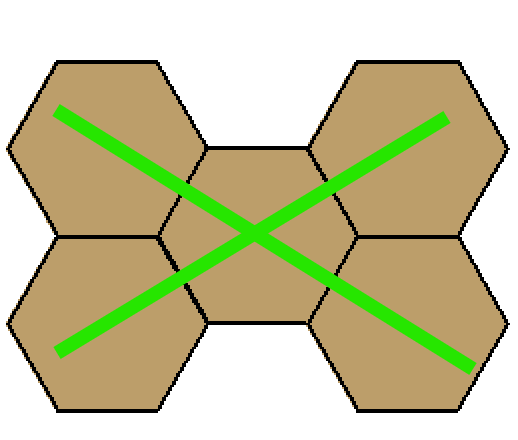
\includegraphics[width=0.75\textwidth]{pictures/tile movability/cross.png}
    \caption{X-shaped blocking configuration.}
    \label{subfig:unmovable_cross}
  \end{subfigure}
  \hfill
  \begin{subfigure}[b]{0.42\textwidth}
    \centering
    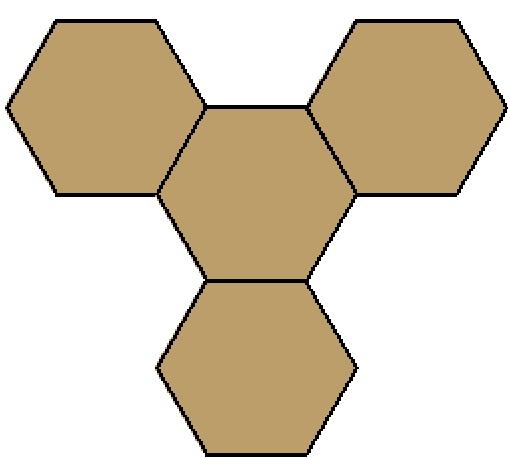
\includegraphics[width=0.75\textwidth]{pictures/tile movability/triangle.png}
    \caption{Triangular blocking configuration.}
    \label{subfig:unmovable_triangle}
  \end{subfigure}
  \caption{The two neighbour configurations that render the central tile unmovable.
    Any rotation of either pattern is equally blocking.}
  \label{fig:unmovable_configs}
\end{figure}



\chapter{Nonaga's Branching Factor Calculation}\label[appendix]{branching}
% Review Iterative Deepening Minimax and Alpha-Beta pruning.
% Discuss Zobrist hashing and state reuse.
The number of possible moves in any Nonaga board state is given by the following equation: \\
\begin{equation}
B = \sum_{i=1}^{3} \sum_{j=1}^{P_i} \sum_{k=1}^{T_{i,j}} D_{i,j,k}
\label{eq:branching_factor_detailed}
\end{equation}

Where:
\begin{itemize}
    \item $B$: The total branching factor (number of possible complete turns from the current state).
    \item $i$: The index of the current player's piece ($i \in {1, 2, 3}$).
    \item $P_i$: The total number of valid destinations for piece $i$.
    \item $j$: The index of a specific destination for piece $i$ ($j = 1, 2, \dots, P_i$).
    \item $T_{i,j}$: The number of legally movable tiles, dynamically evaluated \textit{after} piece $i$ has been moved to destination $j$.
    \item $k$: The index of a specific movable tile ($k = 1, 2, \dots, T_{i,j}$).
    \item $D_{i,j,k}$: The number of valid placement destinations for tile $k$, given the board configuration resulting from move $j$.
\end{itemize}
To determine the initial branching factor, the calculation can be simplified by exploiting the symmetrical nature of the board on all 3 axis of the central hexagon. First, $D_{i,j,k}$ is the same for all $i,j,k$. Second, calculating the branching factor for only one piece and then multiplying the result by three results in the branching factor of the position. Third, for each piece two moves yield the same number of movable tiles.\\
Calculating the number of tile moves for 2 piece moves, multiplying one of them by 2 and adding it to the other results in all possible piece and tile moves for one piece and multiplying that number by three results in the branching factor of the position.
\begin{figure}[H]
    \centering
    % --- First Figure ---
    \begin{minipage}{0.49\textwidth}
        \centering
        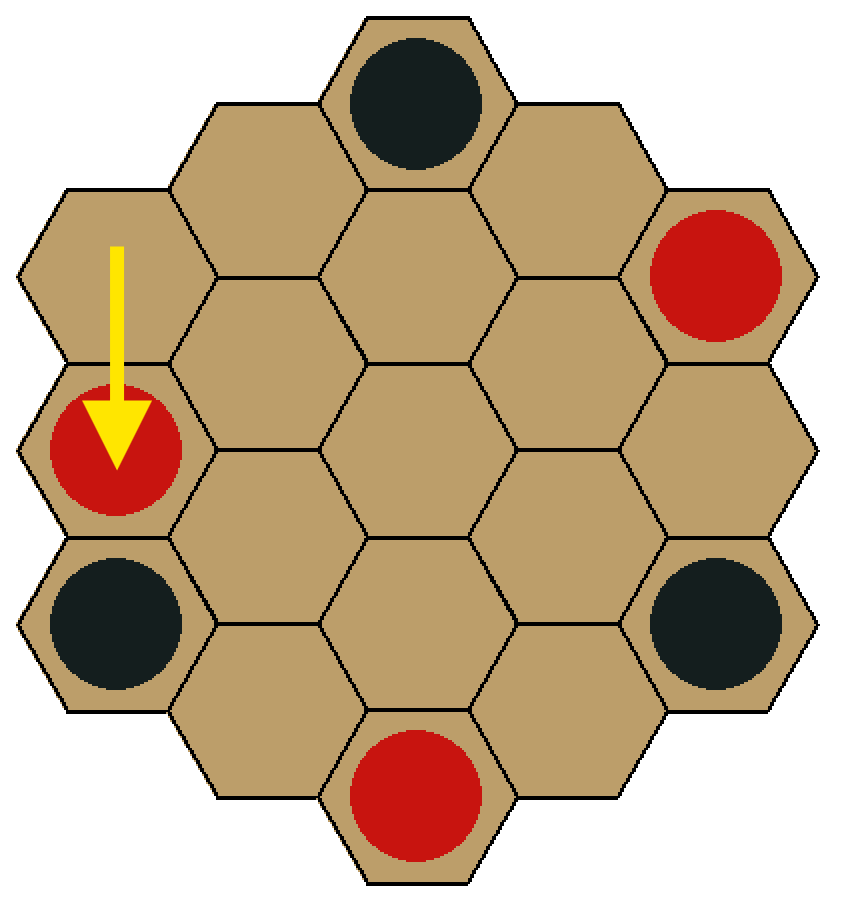
\includegraphics[width=0.42\textwidth]{pictures/init pos/starting piece move to movable.png}
        \caption{Piece move selected.}
        \label{fig:starting piece move to movable}
    \end{minipage}\hfill
    % --- Second Figure ---
    \begin{minipage}{0.49\textwidth}
        \centering
        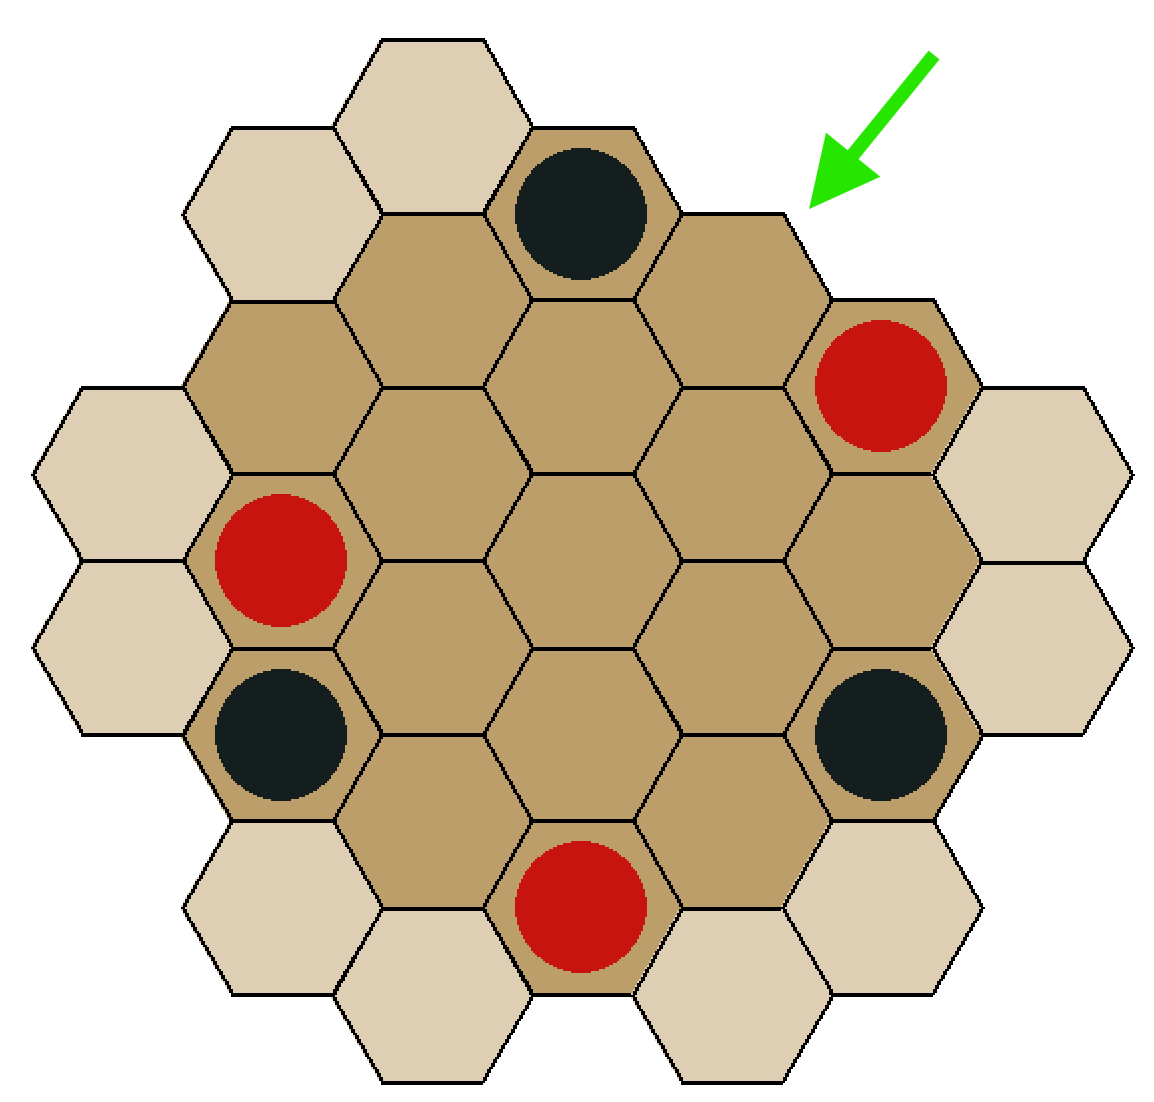
\includegraphics[width=0.58\textwidth]{pictures/init pos/starting tile moves after movable.png}
        \caption{Possible tile moves after the piece move in \cref{fig:starting piece move to movable} of the tile pointed to}
        \label{fig:starting tile moves after movable}
    \end{minipage}
\end{figure}
After the piece move in \cref{fig:starting piece move to movable}, the total number of possible tile moves, as seen in \cref{fig:starting tile moves after movable}, is $NumOfTiles*D = 6*10=60$. It is identical to the total number of possible tile moves after the piece move in \cref{fig:starting piece move to movable 2}. It is doubled to get the number of possible tile moves for both moves.
\begin{figure}[H]
    \centering
    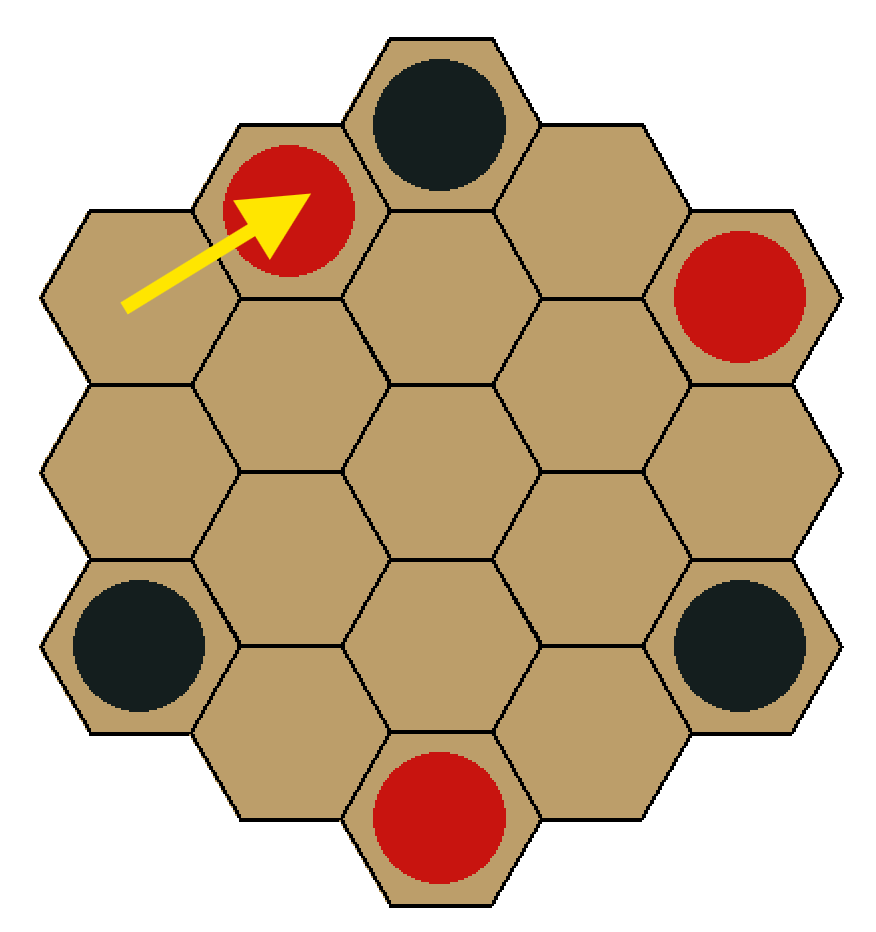
\includegraphics[width=0.235\textwidth]{pictures/init pos/starting piece move to movable 2.png}
    \caption{The piece move with the same number of tile moves as the one in \cref{fig:starting piece move to movable} }
    \label{fig:starting piece move to movable 2}
\end{figure}
\begin{figure}[H]
    \centering
    % --- First Figure ---
    \begin{minipage}{0.45\textwidth}
        \centering
        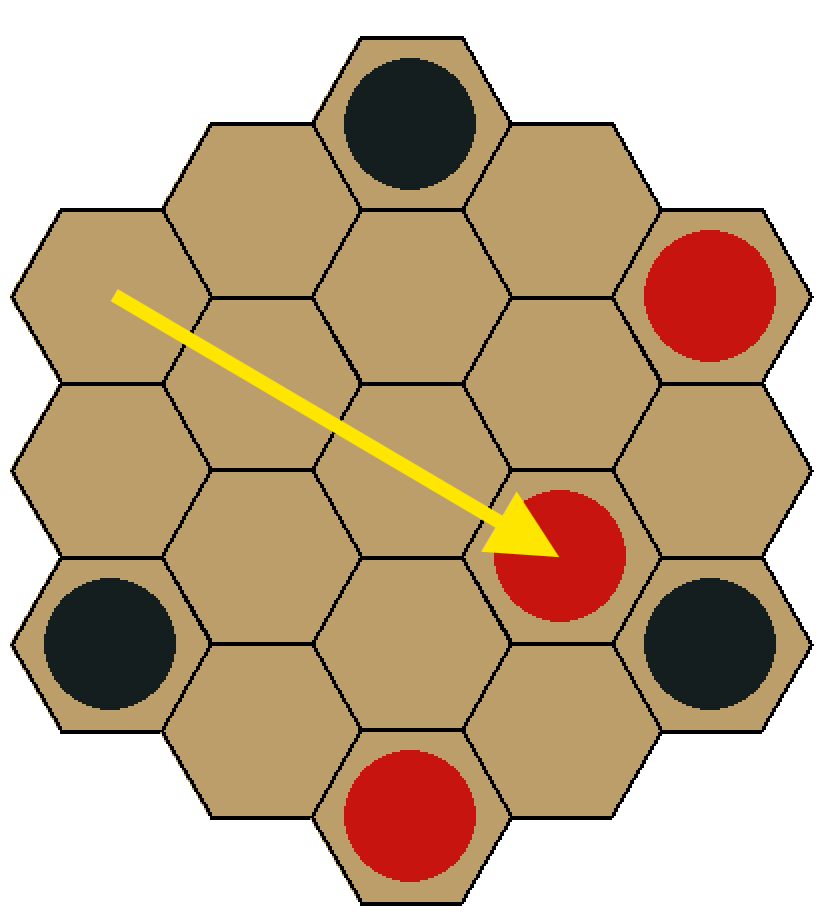
\includegraphics[width=0.43\textwidth]{pictures/init pos/starting piece move to unmovable.png}
        \caption{The last piece move to consider}
        \label{fig:starting piece move to unmovable}
    \end{minipage}\hfill
    % --- Second Figure ---
    \begin{minipage}{0.45\textwidth}
        \centering
        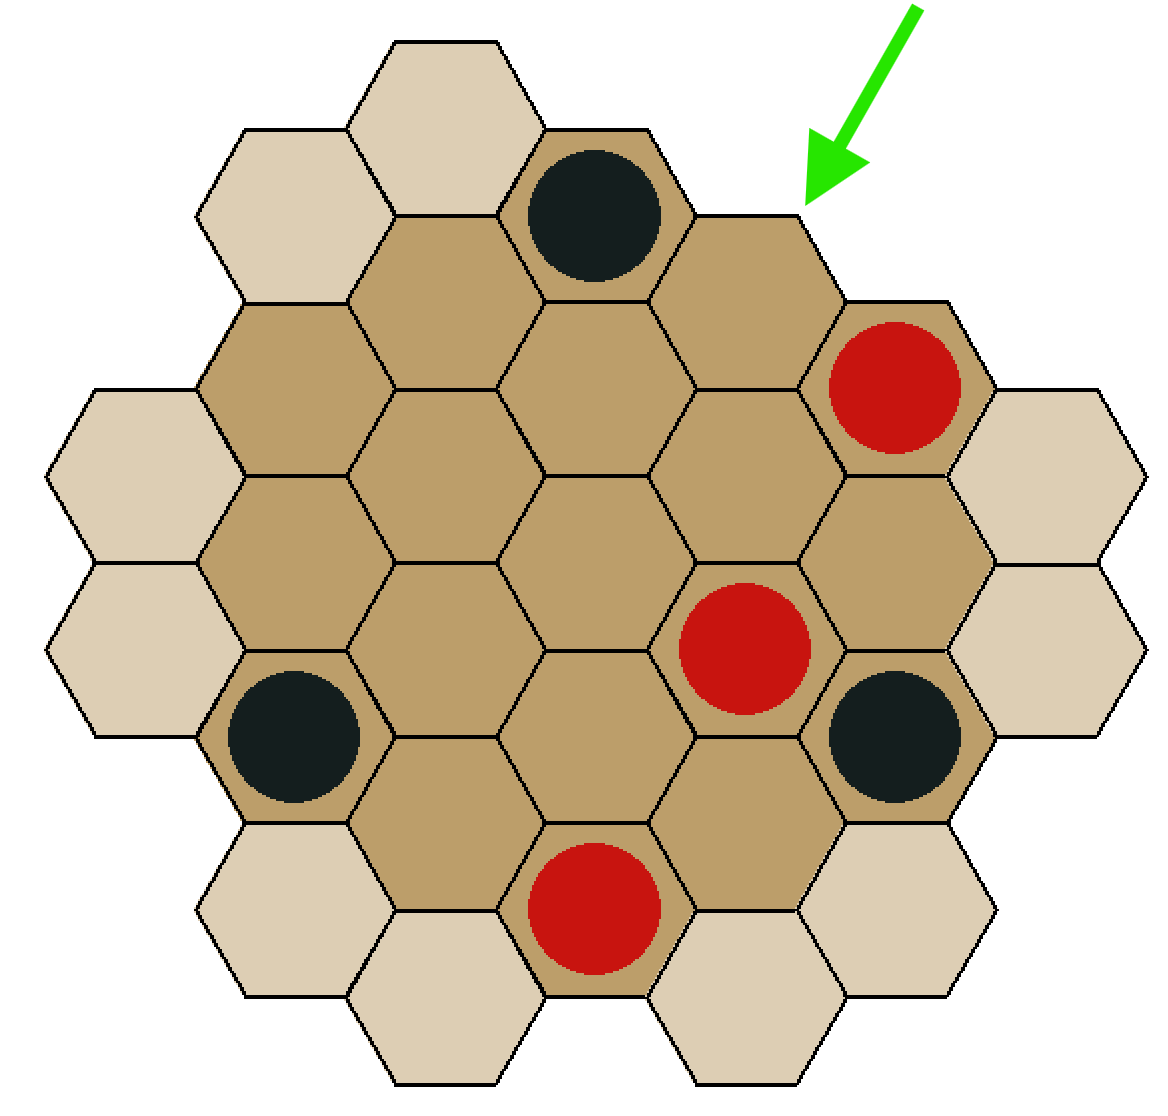
\includegraphics[width=0.60\textwidth]{pictures/init pos/starting tile moves after unmovable.png}
        \caption{Possible tile moves after the piece move in \cref{fig:starting piece move to unmovable} of the tile pointed to}
        \label{fig:starting tile moves after unmovable}
    \end{minipage}
\end{figure}
After the piece move shown in \cref{fig:starting piece move to unmovable}, the total number of possible tile moves (\cref{fig:starting tile moves after unmovable}) is calculated as $N_{\text{tiles}} \times D = 7 \times 10 = 70$. Consequently, the total number of valid moves for the starting position is $3 \times (60 \times 2 + 70) = 570$.While the starting position provides a theoretical maximum, empirical analysis of middle-game states indicates an effective branching factor ($b$) of approximately 440. This reduction occurs because pieces become tightly packed as the game progresses, physically restricting their valid movement vectors. A branching factor of 440 is exceptionally high. For context, Chess has an average branching factor of approximately 35 \cite{Artificial_intelligence}, and Go, a game long considered a grand challenge for AI until the advent of AlphaGo in 2016 \cite{Go_Paper}, averages around 250. However, evaluating a game's computational difficulty requires analysing the overall game-tree complexity, approximated as $O(b^d)$, where $d$ is the average game depth. While Nonaga's branching factor is roughly 12.5 times larger than that of Chess, a typical game of Nonaga lasts for only about 15 moves. In contrast, Chess averages around 40 full moves (80 plies) and Go extends to roughly 150 moves. Therefore, despite the dense move generation at any individual node, the shallow depth of Nonaga significantly truncates the overall search space. This specific structural characteristic makes the game highly suitable for the Iterative Deepening Minimax architecture with Alpha-Beta pruning implemented in this project, as terminal or highly-evaluable states can be reached within a computationally feasible horizon.



\chapter{Brute-Force Feasibility Analysis}
\label[appendix]{sec:hpc_feasibility}

A suggestion raised development ~\cite{assessor} was to evaluate whether
exhaustive enumeration of the evaluation-function weight space, potentially parallelised
on the University of Leeds AIRE HPC cluster, could have served as a viable alternative to
the GA. This section discusses the computational and theoretical infeasibility of that approach.

The evaluation function is parameterised by eight integer weights $w_i \in [0, 50]$,
yielding a search space of $51^8 \approx 1.885 \times 10^{13}$ distinct vectors. Even
under a severely restricted apex-gene formulation capping each weight at $[1, 6]$,
the candidate space is $6^8 = 1{,}679{,}616$. Evaluating each candidate requires playing
it against at least one opponent. Using the 20-game tournament protocol employed by the
GA and a representative game duration of 20~seconds, the total sequential compute time is:
\[
  1{,}679{,}616 \times 20 \text{ games} \times 20 \text{ s/game}
  \;\approx\; 672 \times 10^6 \text{ s}
  \;\approx\; 21 \text{ years.}
\]
Parallelising across the 46 available AIRE cores reduces this to approximately 169~days,
still far exceeding both the project timeline and the available HPC allocation. For the
full $[0, 50]^8$ domain the figure is larger by a factor of $(51/6)^8 \approx 11{,}200$,
rendering the problem cosmologically infeasible in any unparalleled regime.

Beyond raw compute time, there is a deeper methodological objection: as discussed in
\cref{GA testing}, a chromosome's fitness is inherently relative to the quality of its
opponents~\cite{rosin1997new}. Evaluating each candidate against a fixed reference agent
would require selecting that reference agent non-trivially, and a poorly chosen reference
would inflate or deflate the fitness of entire candidate subspaces. The GA sidesteps this
by co-evolving a diverse population, which constitutes the principled and
well-established solution to the relative-fitness challenge in adversarial game
playing~\cite{ficici2000game}.

The brute-force analysis therefore confirms that the GA is not merely a pragmatic
shortcut but the methodologically appropriate approach to this problem class, delivering a
practical convergence in hours rather than centuries while managing the relative-fitness
challenge inherent to game-theoretic parameter optimisation.





\chapter{Benchmark Implementation}

\section{Benchmarking Harnesses Variations}
\label[appendix]{subsec:version_feature_benchmarking_variations}
First, the Final Engine Benchmark
wraps each search call in Python orchestration code (game-state management,
move selection, and logging) so the measured time includes Python overhead that the
Engine Improvement Benchmark excludes by timing only the inner C minimax kernel. \\
Second, the Final Engine Benchmark
accumulates nodes across all iterative-deepening passes (depths~1 through~$d$);
the shallow passes contribute many rapid, low-node calls to the elapsed-time denominator
while contributing relatively few nodes to the numerator, which suppresses the reported
NPS.



\end{appendices}
